\section{Training Data Generation}
Our approach exploits structural information like \FB \CVT tables to  automatically annotate event mentions\footnote{An event mention is a
phrase or sentence within which an event is described, including its type and arguments.} in order to generate training data to learn an
event extractor. Such an approach is known as Distant Supervision~\cite{mintz2009distant}. Essentially, we use the knowledge extracted from
a known knowledge base to \emph{distantly supervise} the process of training data generation using another dataset.


We use the arguments of a \CVT table entry to infer what event a sentence is likely to express. A \CVT table entry can have multiple
arguments but not all of the arguments are useful in annotation. For example, the \texttt{divisions\_formed} argument in
Figure~\ref{fig:example} (b) is not as important as the other three arguments when determining if a sentence expresses a
\texttt{business.acquisition} event. Therefore, our first step is to identify the key arguments from a \CVT table entry. A \textbf{key
argument} is an argument that plays an important role in one event, which helps to distinguish with other events. If a sentence contains
all key arguments of an entry in an event table (e.g. a \CVT table), it is likely to express the event expressed by the table entry. If a
sentence is labelled as an event mention of a \CVT event, we also record the words or phrases that match the entry’s properties as the
involved arguments, with the roles specified by their corresponding property names. For instance, sentence S1 shown in
Figure~\ref{fig:example} (a) is a mention of \texttt{business.acquisition} type, its involved arguments are ``Remedy Corp", ``BMC
Software", and ``2004", and the roles of the three arguments are \texttt{company\_acquired}, \texttt{acquiring\_company} and \texttt{date}
respectively.

In addition to use the raw information given by a \CVT entry, we also use alias information (such as Wikipedia redirect) to match two
arguments that have different literal names but refer to the same entity (e.g. Microsoft and MS).

\subsection{Determining Key Arguments}
We use the following formula to calculate the importance value, $I_{cvt, arg}$, of an argument \emph{arg} (e.g., date) to its event type
\emph{cvt} (e.g., \texttt{business.acquisition}):

\begin{equation}
	I_{cvt, arg} = log \frac{count(cvt, arg)}{count(cvt) \times count(arg)}
\end{equation}


where $count(cvt)$ is the number of instances of type $cvt$ within a \CVT table, $count(arg)$ is the number of times $arg$ appearing in all
\CVT types within a \CVT table, and $count(cvt, arg)$ is the number of $cvt$ instances that contain $arg$ across all \CVT tables.
\FIXME{explain how do you come up with this formula.}


Our strategy for selecting key arguments of a given event type is described as follows:

\begin{description}

\item [P1] For a \CVT table with $n$ arguments, we first calculate the important value of each argument. Next, we sort the arguments
    according to their importance values in descending order, so that arguments with the highest importance values will appear on the top
    of the list. We then consider the top half $\ceil[\big]{n/2}$ (rounding up) arguments on the sorted list as key arguments.

\item [P2] We find that time-related arguments are useful in determining the event type, so we always include time-related arguments
    (such as date) in the key argument set.

\item [P3] We also remove sentences from the generated dataset in which the dependency distances between any two key arguments are
    greater than 2.

\end{description}

Using this strategy, the first three argument of the CVT entry are considered to be key arguments for event typ
\texttt{business.acquisition}.


\subsection{Key Argument Selection Parameters}
To determine how many arguments should be chosen (step P1 in our strategy), we have conducted a series of evaluations on the quantity and
quality of the datasets using different policies. We found that choosing the top half arguments (sorted by their importance scores) gives
the best accuracy for event labeling.

We use three example sentences from the Wiki text dataset to explain steps P2 and P3 in our key argument selection strategy described
above. The three sentences are:

\begin{quote}
\textbf{S2}: \underline{\emph{Microsoft}} spent \$6.3 billion buying online display advertising company \underline{\emph{aQuantive}} in
\underline{\emph{2007}}.
\end{quote}
\begin{quote}
\textbf{S3}: Microsoft hopes aQuantive's Brian McAndrews can outfox Google.
\end{quote}
\begin{quote}
\textbf{S4}: On April 29th, Elizabeth II and Prince Philip witnessed the marriage of Prince William.
\end{quote}

\begin{table}
 \scriptsize
 \caption{\CVT entry of \texttt{business.acquisition} in \FB. \label{tbl:bs}}
        \begin{tabular}{llllc}
        \toprule
        id & company\_acquired & acquiring\_company & date & divisions\_formed\\
        \midrule
        m.05nb3y7 & aQuantive & Microsoft & 2007 & N/A\\
        \bottomrule
        \end{tabular}
\end{table}


\begin{figure}
\centering
	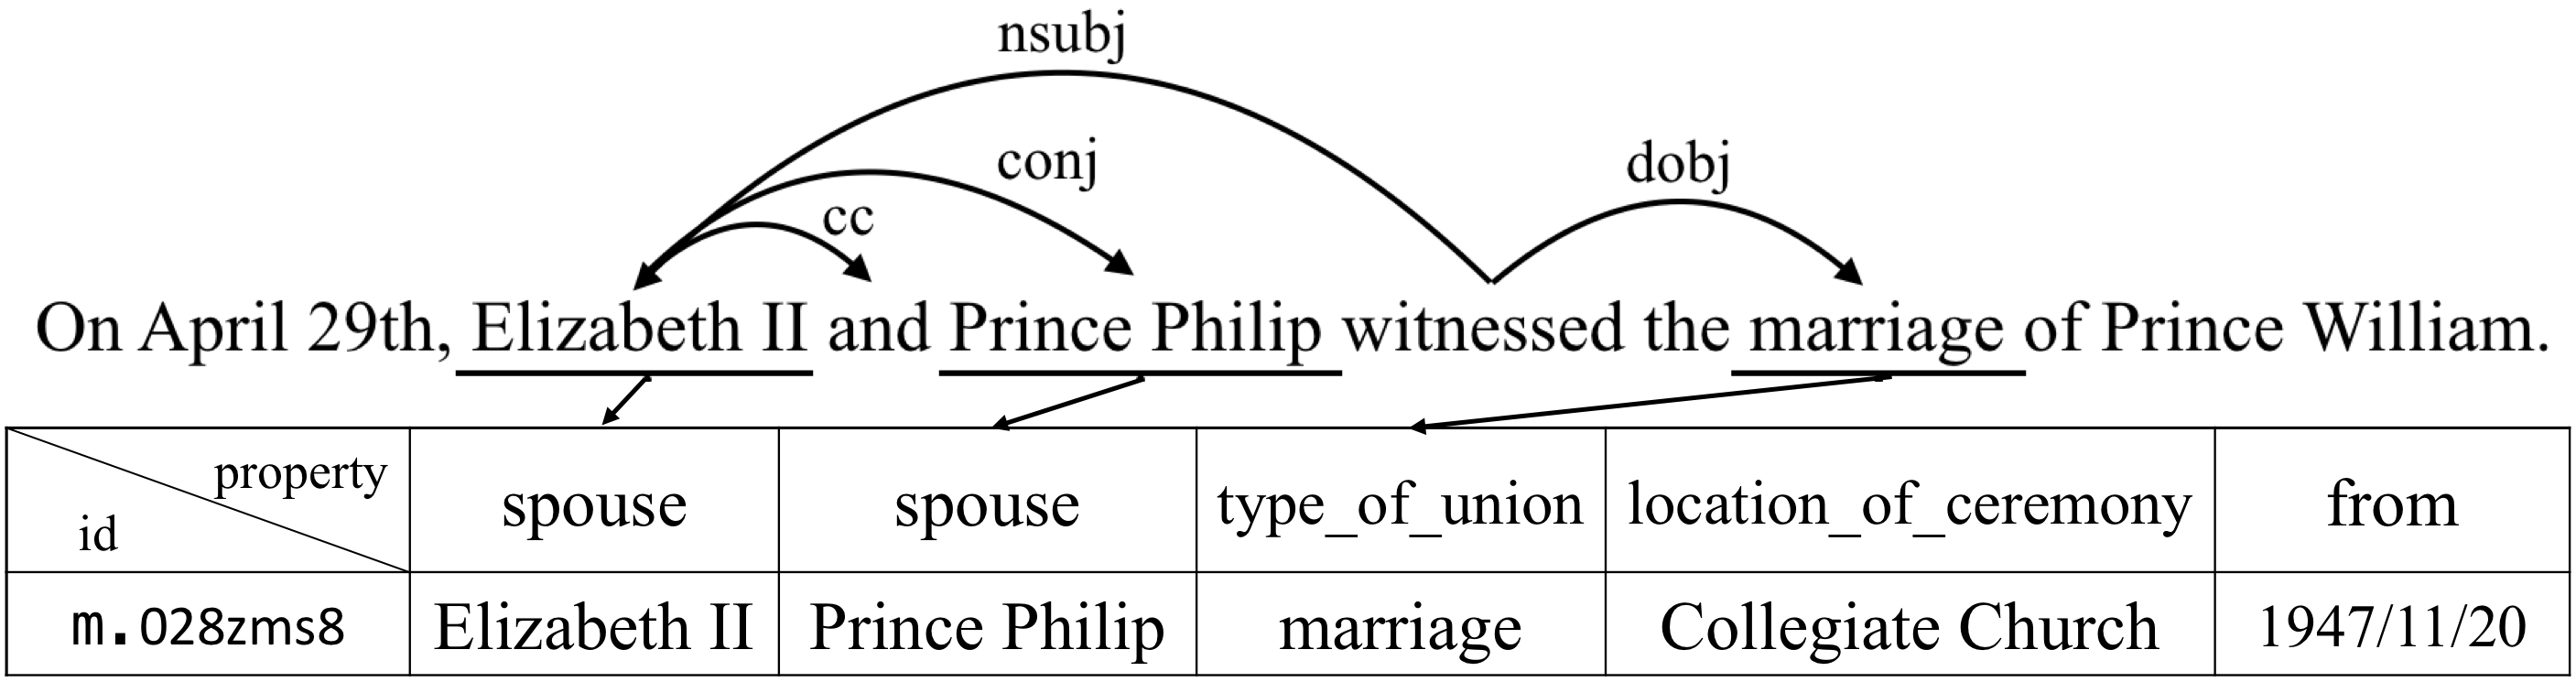
\includegraphics[width=.48\textwidth]{figure2.png}
	\caption{The dependency tree of S3, which partially matches a \CVT entry of \emph{people.marriage} from \FB. \label{fig:2}}
\end{figure}


Although time-related arguments are often missing in the currently imperfect \KBs, they are crucial to identify the actual occurrence of an
event. As an example, suppose we want to use the \CVT entry shown in Table~\ref{tbl:bs} to determine if sentence S3 is a
\texttt{business.acquistion} event. This sentence contains \emph{Microsoft} as \texttt{acquiring\_company} and \emph{aQuantive} as
\texttt{company\_acquired}. If we ignore the time-related argument (i.e., date in this case), this setence could be mistakenly considered
as a positive sample for event \texttt{business.acquisition}. Therefore, we always consider time-related arguments as key arguments (step
P2) if these are given on the \CVT entry.

Finally, step P3 is based on our intuitions that two arguments involved in the same event mention are likely to be closer within the
syntactic structure. As an example, consider S4. The dependency parse tree of this sentence is given in Figure~\ref{fig:2}. As can be seen
from the diagram, although both \emph{Prince Philip} and \emph{marriage} can be matched as key arguments in a  \texttt{people.marriage}
entry, but with a distance of 3 (i.e., far from each other under our criterion) on the dependency parse tree, thus S4 will be labelled as
negative.

\subsection{Data Generation}
To generate training data, we follow a number of steps. Our approach takes in existing structured tables or lists that are organized in a
way similar to the \FB \CVT tables. The structured tables can be obtained from an existing knowledge base, created by experts, or generated
through a combination of both approaches. For each event type, we determine the key arguments for each entry within that type used the key
argument selection strategy described above. This step produces a set of rules to be used for data labeling, where each rule contains the
event type, key arguments and non-key-arguments given by a structured table entry.

Next, we label each individual sentence from the target dataset. The labeling process  is straightforward. We enumerate all rules from the
generate rule set, and check if the target sentence contains all the key arguments specified by a rule. We regard a sentence as a
\emph{positive} sample if it contains all the key arguments of a rule, or \emph{negative} otherwise. For example, S1 in Figure~\ref
{fig:example} (a) and S2 (with its arguments in italics and underlined) are positive examples, while S3 and S4 are negative.

Finally, we tag each word of the sentence using the standard begin-inside-outside (\texttt{BIO}) scheme\FIXME{\cite{}}, where each token is
labeled as \texttt{B-role} if it is the beginning of an event argument with its corresponding role \texttt{role}, or \texttt{I-role} if it
is inside an argument, or \texttt{O} otherwise. We call this a labelling sequence. For instance, Figure~\ref{fig:ls} illustrates the
labeling sequence for sentence S1 given in Figure~\ref{fig:example} (a).  As an output, we record the raw text of each training sentence,
plus its labeling sequence, and key and non-key arguments.

\begin{figure}[t!]
\centering
\scriptsize
\begin{tabular}{ccccccc}
\toprule
Remedy & Corp & was & sold & to & BMC & \\
\rowcolor{Gray} \texttt{B-com.\_ac.} & \texttt{I-comp.\_ac.} & \texttt{O} & \texttt{O} & \texttt{O} & \texttt{B-ac.\_comp.} &\\
\end{tabular}
\begin{tabular}{ccccc}
Software & as & the & Service &Management \\
\rowcolor{Gray} \texttt{I-acq.\_comp.} & \texttt{O} & \texttt{O} & \texttt{div.\_form.} & \texttt{div.\_form.} \\
Business & Unit & in & 2004 &.\\
\rowcolor{Gray} \texttt{div.\_form.} & \texttt{div.\_form.} & \texttt{O} & \texttt{B-date} &\\
\bottomrule
\end{tabular}

\caption{The labeling sequence for sentence S1 shown in Figure~\ref{fig:example} (a). Each token of the sentence is tagged using the \BIO
scheme. \label{fig:ls}}
\end{figure}

\subsection{Limitations}
Our approach relies on structured tables or lists to automatically label text. The table can be obtained from an existing knowledge base or
hand-crafted by developers. We stress that providing a table incurs much less overhead than manually tagging each training sentence, as a
single table entry can be automatically applied to an unbounded number of sentences.  Moreover, like all supervision-based event
extractors, our approach does not support detecting new event types that are not seen in the training data. However, our approach does
offer an easy way to extend the structured table to support new types, i.e., by adding new entries to the table.


Our current implementation does not disambiguate pronouns. There are co-reference methods\FIXME{~\cite{}} that can be used to find out
which word a pronoun refers to. These works are therefore complementary to our approach. Integrating our work with co-reference methods is
our future work. Furthermore, our approach targets at sentence-level event detection. There are methods like \FIXME{\cite{}} can be used to
extend our approach to document-level event extraction.
